\section{Implementation}
\label{sec:impl}

Below we describe our implementation of \this{}'s key components.

\subsection{Performance and Scalability}
\label{sec:perf}

The goal of Rust is to provide memory safety without sacrificing performance by implementing a set of rule checking mechanism which is designed to prevent memory related bug. Therefore, the final program is free of the related bugs. \this{} also uses Rust's design. We compare the performance of \this{} and PMDK~\cite{pmdk} in \refsec{sec:results}. However, the performance of \this{} depends on several factors.

\begin{itemize}
    \item Memory management is generic in \this{}. We provide a standard implementation of a Buddy Block allocator which can be used to define new \csym{MemPool}s. However, the programmer may develop a custom allocation mechanism which may or may not be faster than our standard allocator.
    \item Log taking is a costly process. Currently, we use an undo log mechanism which takes log of data only when it is necessary. \this{} is designed in a way that the Rust compiler will warn about unnecessary log taking and transactions. Even if the programmer mistakenly borrow a mutable reference to the object, \this{} does not take log until data is dereferenced mutably (while writing to). \this{} also takes log of data once per transaction.
    \item Log sizes is an important performance issue which it is determined by the programmer. For example, one can wrap a whole array of 1024 elements in a \csym{LogCell} and take log of the array entirely while mutably access it. This might be a good implementation depending on the application. However, if a single element is going to be updated, it is better to have an array of 1024 elements individually wrapped in a separate \csym{LogCell}. Thus, although the programmer does not need to take care of memory-safety, s/he is responsible for the performance.
    \item The underlying device determines how fast can we operate on it. This is out of both \this{}'s and the programmer's control.
    \item The recovery procedure in \this{} is fast as it only need to restore the leftover logs without scanning the entire system.
\end{itemize}

We have designed \this{} to support petabytes of data, and the internal memory usage is a fixed number. \this{} also can be used on any type of storage system as long as a DAX filesystem can run on top of it. The performance of \this{} crate is a factor of the size of transactions and not the size of the device. In case of using a block device rather than a byte addressable persistent memory, \this{} should be configured with a flag that forces it to use \msync{} instead of a write barrier. 


\subsection{Memory Allocation}
\label{sec:mem-alloc}

\This{} uses a persistent buddy allocator that includes features
to provide scalability and support for \this{}'s transactional interface.  Most
of it is implemented in normal Rust, but the low-level allocation code (which
programmers do not interact with directly) is unsafe.

The allocator keeps a free lists for each power-of-two size of memory chunk starting at 8 bytes.  On allocation it searches the list that holds the smallest chunks that could hold the requested space.  If the list is empty, it splits a chunk from the next smallest free list.  The allocator maintains one set of free lists for each core to minimize contention.

The allocator works with the transaction system to ensure leak-free memory allocation.  During a transaction, the allocator logs memory allocation operations internally.  After a crash, the allocator rolls back the operations if the transaction had not committed.  Otherwise, replays the allocations to complete them and make them persistent.  A similar mechanism applies to deallocations.


\ignore{
We
integrate a fast, self-contained, atomic memory allocator in \this{} by
implementing \textit{buddy allocation} algorithm, all packed in \csym{BuddyAlloc} type. It is self-contained because it does not use any resources other than the pool itself to keep its metadata information.  It is also failure-atomic which means that the whole process of allocation/deallocation is reversible in case of a crash. We also make it thread-safe by \steve{providing each core with a separate allocator, and} guarding the operations with a spin-lock \steve{to prevent data race when one core attempts to use another core's qouta due to lack of space}.}

\ignore{\subsubsection{Allocation algorithm.} We implement buddy-block algorithm to provide fast and efficient memory allocation. The allocator consists of 61 sorted linked-lists for free memory blocks of sizes between $2^3$ and $2^{64}$ bytes ($\lst_3..\lst_{64}$). Because we use the first 8 bytes of every free block as a pointer to the next free block, a block cannot be smaller than 8 bytes.
To \textit{allocate} $n$ bytes, we first search $\lst_{\lceil \text{log}~n\rceil}$ for a free block with the size of the smallest power of two that is larger or equal to $n$. If there is no such block, the allocator searches for the next smallest power of two in $\lst_{\lceil \text{log}~n+1\rceil}$ and splits it in two halves. Then, it uses the first one and puts the second one in $\lst_{\lceil \text{log}~n\rceil}$. The allocator recursively reiterates this process on $\lst_i$ where $\lceil \text{log}~n\rceil < i \le \lfloor \text{log}~size \rfloor $ until either it finds a free block or memory exhausts.
To \textit{deallocate} address range of $[a,a+n)$, we should put a free block back to $\lst_{\lceil \text{log}~n\rceil}$. However, if there is a buddy block in the same list, which can be either $[a-n,a)$ or $[a+n,a+2n)$, they merge together to provide a larger free block which is either $[a-n,a+n)$ or $[a,a+2n)$ in $\lst_{\lceil \text{log}~2n\rceil}$. We recursively reiterate the process until no buddy block is found.}

   \ignore{       

\subsubsection{Two-level atomicity.} Since the memory allocation is subject to crashes, we consider a \textit{low-level} atomicity for the metadata consistency, as opposed with the \textit{high-level} atomicity in which the allocation is assumed to be failure-atomic and the reversibility is guaranteed through \csym{DropOnCommit} and \csym{DropOnFailure}. In the low-level atomic section, we log the required updates to the buddy lists in a fixed size auxiliary buffer. At the end of the atomic section, we start draining the buffer and applying the changes to realize the allocations. When a crash happens, we first finish draining the buffer, then, we use the low-level drop logs to revert the operation.
%Note that the low-level drop logs are different from the high-level logs. Low-level logs are limited in quantity and they are used only when a crash happens in the middle of memory allocation/deallocation to protect metadata. The high-level drop logs are unlimited and they are used when a crash happens in a high-level transaction to prevent memory leaks and pointer-related bugs.
\reflst{lst:llatom} shows how the low-level atomicity is used to avail high-level reversibility. At line 3, a new memory block is temporarily allocated in low-level logs. At line 4, we allocate a high-level log for reversibility. Although we record all required changes to the allocator, none of the allocations realizes until the end of the atomic section. If a crash happens, depending on the completeness of the low-level atomic section, we decide to whether realize the allocations, or discard the low-level logs.

\begin{lstlisting}[caption={Atomic allocation},label={lst:llatom}]
fn new<T>(x: T, j: &Journal) -> &mut T {
    Self::atomically(||{
        let p = Self::new_nolog(x);
        Log::drop_on_failure(p, j);
        p
    })
}
\end{lstlisting}
}

Programs cannot invoke the allocator directly.  Instead, they invoke the \csym{new} method of \csym{Pbox<T>}, \csym{Prc<T>}, or \csym{Parc<T>}.  Deallocation occurs when a \csym{PBox} goes out of scope or the reference count for a \csym{Prc} or \csym{Parc} goes to zero.

\ignore{
\subsubsection{Allocation interface.} To protect memory management subsystem from corruption, low-level operations are not available to the user. Instead of that, \this{} provides three persistent pointer type wrappers (i.e. \csym{Pbox<T>}, \csym{Prc<T>}, and \csym{Parc<T>}) that allows dynamic allocation and deallocation through RAII. \steve{These type wrappers have the same properties as Rust's standard pointer wrappers which are described in \refsec{sec:wrapper}, except that they internally manage persistence safety, and they accept a \csym{NVSafe} type for data (\csym{T}) and a pool type \csym{P}}. The constructor methods use the \csym{new} function (\reflst{lst:llatom}) to allocate memory which guarantees reversibility on failure. The destructor method only allocates a \csym{DropOnCommit} log for the data. As they describe themselves, they drop the allocation for data depending on the transaction's status, atomically.
}



\subsubsection{Data Race Prevention}
\label{sec:no-race}

Inherited from Rust, \this{} guarantees an absence of data races. The general form of data race which might happen by aliasing a mutable reference is impossible in Rust. Therefore, the programmer may not send a mutable reference to a thread. However, interior mutability allows threads to mutably borrow data from immutable references. To prevent multiple mutable references in multiple threads, \this{} marks \csym{LogCell} and \csym{LogRefCell} as not being \csym{Send} and \csym{Sync}. However, \csym{Mutex} allows synchronously obtaining a mutable reference to the shared data once at a time, so it is \csym{Send} and \csym{Sync}.

Another undesirable data race may happen while updating the reference counters in \csym{Prc}. To prevent that, \this{} uses atomic counters in \csym{Parc} and disallows \csym{Prc} to be sent or shared between threads. Prevented by trait bounding, the only possible way to have share data of type \csym{T} between multiple threads is to use \csym{Parc<Mutex<T>{>}} (or other arrangements of them).


\subsection{Transactions}
\label{sec:mutex}

\subsubsection{Isolation}

In PM programming, it is not enough to synchronize mutable accesses to data, because releasing the lock after the mutation does not prevent another threads to acquire it, update data, and persist it before the current thread finalizes the transaction (\reffig{fig:mutex}). Additionally, it is possible that the system take double undo logs for the same data, and the the recovery procedure becomes nondeterministic. To prevent that, our \csym{Mutex} locks data throughout the whole transaction and allows re-entrance from the same thread to prevent deadlock.

\begin{figure}%[!ht]
    \begin{center}
    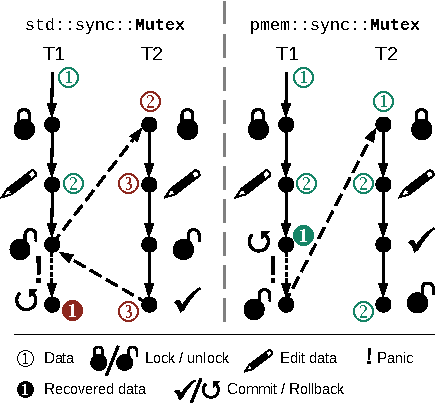
\includegraphics[width=3in]{Figures/tramutex.pdf}
    \end{center}
    \caption{\label{fig:mutex} {\bf Volatile and Persistent Mutex.} As shown on the left, standard \csym{Mutex} may lead to an inconsistent state by rolling back the incomplete transaction after letting data be updated and committed in another thread. On the right, persistent \csym{Mutex} locks data throughout the transaction's lifetime until it finishes to guarantee data consistency.}
\end{figure}

\subsubsection{Unstable Features}

Rust has a sophisticated system for allowing programmers to opt-in to
experimental language features.  Many (but not all) of the experimental
features eventually find their way into the official language.  Our
implementation of \this{} relies on several of these experimental features, but
none of them are fundamental to \this{}'s design: \csym{untagged\_unions}, \csym{specialization}, \csym{optin\_builtin\_traits}, \csym{llvm\_asm (for c lflush\_opt and low level stuff)}, \csym{core\_intrinsics}, \csym{negative\_impls}, \csym{const\_generic\_impls\_guard}, and \csym{const\_generics}.


%% Memory leaks and related pointer bugs are common problems in programming
%% systems when a piece of memory becomes unreachable or unavailable. We address
%% these issues by implementing persistent pointer type wrappers that protect data
%% and the memory management subsystem. \reftab{tab:types} lists the three
%% persistent pointer wrappers. These pointer wrappers share four characteristics
%% for safety: 1) their constructors}/destructors are transactional in order to
%% avoid memory leaks; 2) they do not provide interior mutability to make sure
%% data does not change in crases; 3) additional to the data type, they require a
%% pool type as a part of the wrapper to enforce pool isolation, and 4) they
%% cannot move out of an atomic section unless they become reachable from the root
%% object.

% \subsection{Persistent Pointer Type Wrappers}
% \label{sec:wrappers}

% Persistent objects and volatile objects do not have much differences other than their memory locations. A volatile object reside in the heap and is referenced by a volatile pointer, and likewise, a persistent object resides in the PM and is referenced by a persistent pointers. Since Rust does not provide persistent pointers, \this{} expands Rust's design by providing the persistent version of Rust's standard pointer type wrappers (\refsec{sec:wrapper}) that protect data from system crashes: \csym{Pbox<T,P>}, \csym{Prc<T,P>}, and \csym{Parc<T,P>}. These type wrappers have the same properties as Rust's standard pointer wrappers which are described in \refsec{sec:wrapper}, except that they internally manage persistence safety, and they accept a \csym{NVSafe} type for data (\csym{T}) and a pool type \csym{P}. 

% \subsubsection{Concurrent Access.} Multiple threads may want to allocate from the PM or release memory. Since the PM is a shared resource, it should be protected against data race. We dedicate an individual allocator over a separate memory chunk to each core in order to mitigate the contention. To allow borrowing memory from another chunk on memory exhaustion, each allocator leverages a fast spin lock. Note that the lock is not effective on local allocations.

%% \subsection{Pointer Safety}
%% \label{sec:pointers}

%% The referential integrity invariant means that all pointers in the course of program execution, point to a valid data. This can be provided by enforcing a set of rules that provably prevent undesirable pointer-related bugs. PM programming shares many of this kind of bugs with heap-based programming model. Fortunately, Rust provides pointer safety for that class of bugs. Inspired by Rust's design, we extend its pointer safety to our persistent smart pointers.

%% \subsubsection{Pointer-Data Coexistence}
%% \label{sec:no-dangl}

%% Dangling pointers appear when the lifetime of a pointer is longer than the lifetime of data it points to. Similarly, memory leaks happen when a pointer dies while its data is still alive and unreachable. Rust prevents the former situation by applying drop chain through enforcing RAII. The latter situation is also not possible in Rust since the deallocation of data is controlled by the owner pointer. However, it may happen in PM programming due to write reordering or a crash in the middle of the drop chain. Our persistent pointer types have the same dropping mechanism as the standard smart pointers, except that they use our atomic, leak-free allocator and their counters (if any) are failure-atomic. By enforcing all changes to a pointer (i.e. construction, destruction, and reassignment) to be transactional, holding pointer-data coexistence invariant is guaranteed.

%% \subsubsection{Non-existance of Wild Pointers}
%% \label{sec:no-wild}

%% The smart pointers in Rust own data, which means that they exclusively control over the data creation and destruction. This feature eliminates the possibility of appearing wild pointers, as the pointer allocates its own data. \This{} guarantees non-existence of wild pointers in a similar way. That is the creation of data happens before the creation of owner pointer. Our allocator guarantees the atomicity of the data allocation by packing the data and a drop log in a single atomic allocation. In case of a failure, either both data and its drop log exist, or none of them do. Therefore, the high-level transaction can revert the allocation on recovery using the drop log, if it exists.

%% \subsubsection{Transactional RAII.} In \this, dynamic allocation is available through persistent pointer wrapper constructors which requires a \csym{Journal} object to perform which trivially enforces their invocation to be inside a transaction. To make the destruction transactional too, we should prevent their invocation from outside a transaction which is non-trivial. This is because of Rust's reliance on RAII which may lead to memory deallocation on data assignments. \this{} promises transactional deallocation by enforcing two invariants: 1) no mutation outside transaction, and 2) there should be a path from the root object to this allocation. The former prevents deallocation due to reassignment, and the latter prevents deallocation due to zero references. \reflst{lst:alloc} shows how allocated object can move out of a transaction. The old value of \csym{root} drops at line 5, and the recently allocated object `\csym{new}' replaces it, all happening inside the transaction.

%% \begin{lstlisting}[caption={Transactional data construction/destruction},label={lst:alloc}]
%% type Root = LogCell<Pbox<i32,P>,P>;
%% let (root,p) = P::open::<Root>("1.pool",0);
%% P::transaction(move |j|{
%%     let new = Pbox::new(1, j);
%%     root.set(new, j);
%% }).unwrap();
%% \end{lstlisting}

%% \subsubsection{Loggable interior mutability.} To prevent data loss, we should make sure that the mutations are recoverable. \refsec{sec:over:log} explains recoverable mutation and why it is important in PM programming. To achieve that, the persistent pointer wrappers do not allow mutable dereferencing. Once initialized in a transaction, interior data cannot change. However, this vastly limits the programmability. As explained in \refsec{sec:over:log}, \this{} provides crash-safe interior mutability though a set of memory cell types (the last two rows of \reftab{tab:types}). In contrast with the persistent pointer types, memory cell types wrap around the actual data. They provide special interface for interior mutability that assures the recoverability by taking undo logs before mutation. For example, in \reflst{lst:alloc}, \csym{root} is a memory cell of type \csym{LogCell} that takes a \csym{DataLog} before mutation at line 5.



%% \ignore{
%%     \subsection{Thread-safe pointers}
%%     \label{sec:thrd-safe}
    
%%     \steve{\csym{Prc} and \csym{Parc} both allow sharing data between multiple owners, and manage memory allocation using reference counting. However, when they are shared between threads, data racing might happen while updating the counters. Therefore, since only \csym{Parc} uses atomic counters, we mark it as \csym{Sync} and \csym{Send} to allow being sent and shared by multiple threads. Remember that both \csym{Prc} and \csym{Parc} use failure-atomic counters which are logged before mutation, but \csym{Parc} additionally uses thread-safe atomic counters.}
%% }



% \subsection{Failure Atomicity}
% \label{sec:atomic}

% \reffig{fig:trans} shows the anatomy of a transaction that provides failure atomicity for updating persistent objects. The low-level operations are integrated into \cfunc{transaction} and \cfunc{borrow\_mut}. The write order is preserved by persisting the logs (using \clflush{}, or \clflushopt{}/\clwb{} followed by a \sfence{}) before mutation. We apply source-data swap~\cite{log-nvmm} while taking a log to save one costly persist barrier after updating data. Depending on the result of executing the transaction's lambda, \this{} commits the changes on success, or rolls back them on failure. Then removes the logs from the journal. If a crash happens, the recovery procedure uses the persisted logs to restore the system back to its state before the transaction. The lambda can capture variables bounded by \csym{TxInSafe}, and may return values marked as \csym{TxOutSafe}. Exclusive availability of a reference to the journal object \csym{j} inside a transaction constraints functions taking it as an argument to be enclosed by a transaction.

% To enforce {\it Ordered Writes} and {\it Recoverable Mutation} invariants, \this{} provides atomic sections through software transactional memory (STM) technique and Rust's borrowing mechanism. Working together, \this{} prevents unrecoverable modification to data by taking an undo log before mutating data and preserving persist order of the logs in an atomic section. \reffig{fig:trans} shows a failure-atomic transaction in which a persistent data changes. As shown in this figure, write ordering preservation is hidden. Since journals are created inside a transaction, functions that take a journal as an argument, such as \csym{borrow\_mut} can only be used inside \csym{transaction}. Also, since the mutable borrow is created in the atomic section, Rust's lifetime checker prevents sending it out of the atomic section which may have consequences otherwise. \this{} is designed in a way that the programmer writes the code while holding the invariants without being aware of them. 


% \subsection{Interior Mutabilty}
% \label{sec:mut}

% Interior mutability means that a variable of a wrapper type allows mutable access to its inner value while the outer wrapper is not mutably borrowed. For example, Rust has a type wrapper called \csym{UnsafeCell<T>} which has a method with the following signature: \csym{UnsafeCell<T>::get(\&self) -> *mut T}. Although the \csym{get} function does not require the variable to be mutable, it returns a mutable raw pointer to its inner data of type \csym{T}. This is unsafe to provide interior mutability for persistent objects unless we make sure that data is logged. By definition, \csym{Pbox}, \csym{Prc}, and \csym{Parc} do not provide interior mutability. In \this{}, there are three other type wrappers that safely expose a mutable reference to the protected data: \csym{LogCell}, \csym{Mutex}, \csym{RwLock}, and \csym{Tramutex}. \csym{LogCell} and \csym{LogRefCell} provide interior mutability via functions \csym{set()} and \csym{borrow\_mut()}, respectively, which take a reference to a \csym{Journal}. Its argument forces the programmer to wrap the code in a transaction. \csym{Mutex}, \csym{RwLock}, and \csym{Tramutex} basically have the same mechanism, but they are used for serialization in multi-thread programming. In \reflst{lst:mut}, \csym{list} is of type \csym{Prc<LogRefCell<List,P>,P>} that wraps a pointer to a \csym{List} object inside a \csym{LogRefCell}. In this case, the pointer can only be read, but the whole wrapped persistent pointer can be mutably borrowed as it is in line 9.

% \begin{lstlisting}[caption={Mutably borrowing a persistent object},label={lst:mut}]
% type Ptr = 
%     MaybeNull<Prc<LogRefCell<Node,P>,P{>}>;
% struct Node { val: i32, next: Ptr }
% struct List { tail: Ptr, length: i32 }
% fn add_element(
%     list: &Prc<LogRefCell<List,P>,P>, 
%     val: i32) {
%     P::transaction(move |j|{
%         let mut list = list.borrow_mut(j);
%         list.tail = Valid(Prc::new(
%             LogRefCell::new(Node{
%                 val, next: Null
%             },j),j));
%         list.length += 1;
%     }).expect("Unsuccessful");
% }
% \end{lstlisting}

% The common use of these types is for wrapping the inner value of these pointer wrappers. \reflst{lst:mut} represents a snippet of code that attempts to add a new element to a linked list residing the \csym{P}. The type \csym{List} consists of an optional persistent pointer to the tail of the list, and the length of the list. A \csym{Journal} object for \csym{P} is created at line 8 when we open a transaction. Line 9 takes an undo log of the list data structure. The log is not for entire list, however, it only keeps the old value of the tail pointer and the length of the list. After taking a log, \csym{borrow\_mut()} returns a mutable reference to the list. Any changes being made from this point on to \csym{list} is recoverable. The key point of this implementation is that there is no unsafe way to make changes. Unlike other persistent libraries in which the programmer should call some kind of logging function at the beginning of the transaction (e.g. PMDK~\cite{pmdk}), in \this{} the log taking process is hidden behind Rust's borrowing mechanism. 


% \subsection{Software Transactional Memory}
% \label{sec:stm}

% Software Transactional Memory (STM) is a common practice to control access to the shared data and protect it from system failure in the persistence context. \this{} also is featured with STM to satisfy the invariants described in \refsec{sec:atomic}. Transactions in \this{} have the following properties.

% \begin{itemize}
%     \item \textit{Log Structured}: Opening a transaction creates a \csym{Journal} object, and this is the only way to obtain a reference to a journal. Therefore, when a function takes a journal object as an argument, it basically means that it can be called only from a transaction.
    
%     \item \textit{Thread/Pool Separated}: Each thread can open one transaction per memory pool. Calling transaction function multiple times is allowed but they all refer to the same \csym{Journal} object.
    
%     \item \textit{Matryoshka Principle}: Nested transactions are allowed, but they are ineffective in committing changes. However, if a panic happens, the exception is propagated up to the top transaction and abort all of them. This allows functions to have their own transactions to make sure that their operations are atomic-safe.
    
%     \item \textit{Returning Results}: Transactions can return data of any type with a constraint that it should implement \csym{TransactionOutSafe} trait. None of the persistent pointer wrappers implements this trait. It means that a persistent object cannot live longer than the transaction unless it becomes reachable by the root object.
    
%     \item \textit{Unique Pool Access}: Since transactions belong to pools, only one type of journal is available within a transaction. This means that allocation from multiple pools is not possible inside one transaction (\reflst{lst:cross}). However, nested transaction from different pools is allowed and safe.
% \end{itemize}

% We applied these restrictions to assure that none of the safety invariants is possibly violated. For more clarification, we first explain our journaling mechanism, and then describe how the STM and journaling mechanisms guarantee the satisfiability of the invariants.

% \subsubsection{Journaling} To track the uncommitted changes to the persistent memory, we should durably record all versions of the data in persistent memory. We use undo-logging which means that \this{} writes the old version of data into a data structure called \csym{Journal} right before making changes to the original data. This process happens once per transaction for every data that is going to be modified.

% There are five types of logs:

% \begin{enumerate}
%     \item \csym{DataLog} is the regular log as described above for undo-logging.
%     \item \csym{DropOnFailure} is created while allocating of new data to be used when a power failure happens for reclaiming the allocation as explained in \refsec{sec:mem-alloc}.
%     \item \csym{DropOnCommit} is made while freeing a persistent object. The log will be used to resurrect the object when the transaction was unsuccessful, or system fails.
%     \item \csym{UnlockOnFailure} is used when a lock is acquired and system fails. To release the locks after recovery, \this{} uses logs of this kind to find them (used in \csym{Mutex} and \csym{RwLock}).
%     \item \csym{UnlockOnCommit} is used to release a lock after committing/rolling back a transaction. It also releases the lock on system failure (used in \csym{Tramutex}).
% \end{enumerate}

% According to our rollback journal model, we should make sure that the logs are persistent before modifying data. Therefore, \this{} issues  \clflush{}/\clflushopt{}/\clwb{} and \sfence{} for every corresponding cache line belonging to the log. By doing this, \this{} makes sure that the subsequent writes are safe (it satisfies `Memory Ordering' invariant).

% \begin{figure}%[!ht]
%     \begin{center}
%     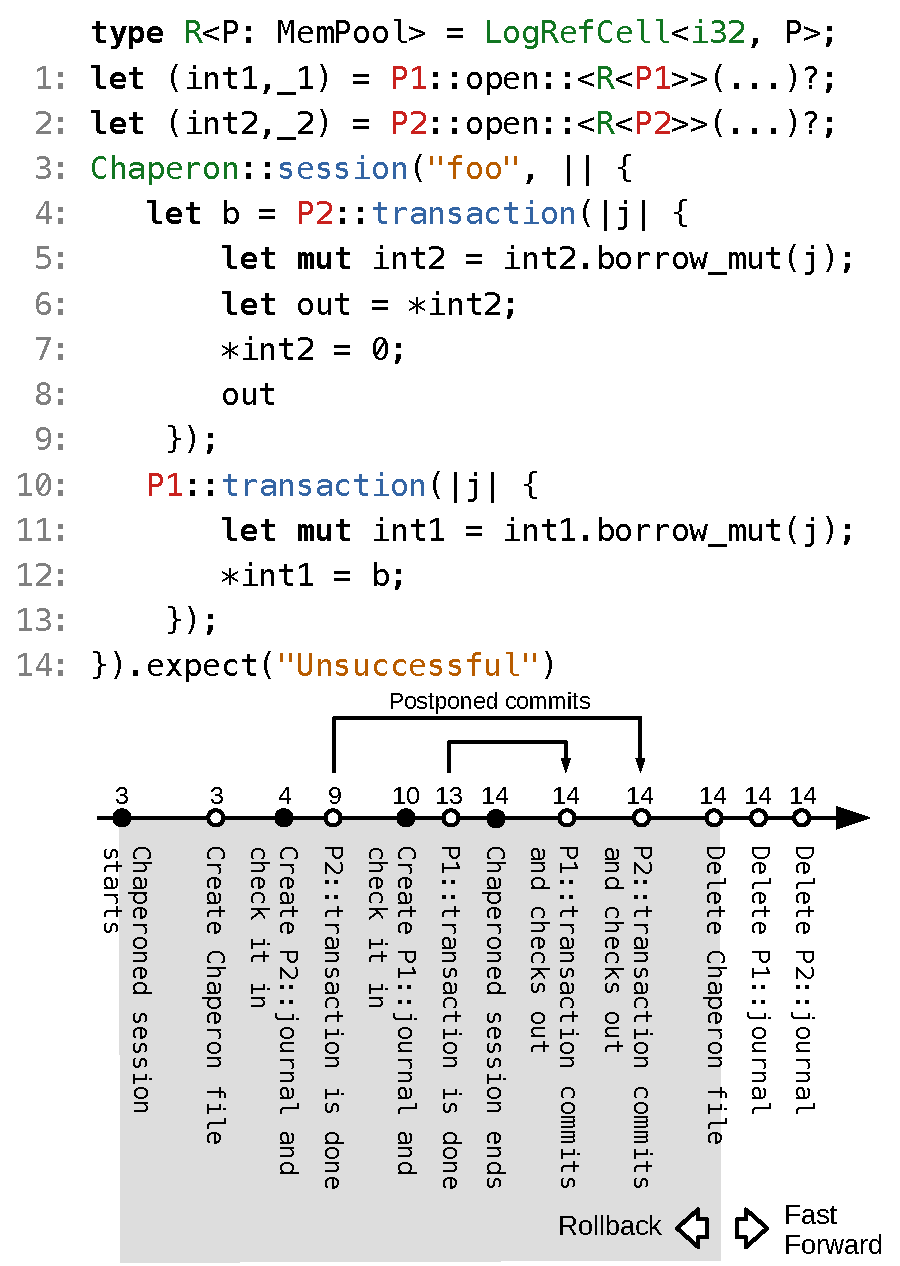
\includegraphics[width=3.2in]{Figures/attach.pdf}
%     \end{center}
%     \caption{\label{fig:cross} {\bf Cross-Pool Transaction.} \csym{Chaperon::session()} provides an atomic section for multiple pools to update persistent objects. The failure atomicity is provided by a separate data structure that monitors all transactions.}
% \end{figure}

% \subsection{Cross Pool Pointers}
% \label{sec:cross-pool}

% \steve{partialy redundant (sec 4.3: Pointers to Persistent Data)}

% To provide persistent memory access, we defined a special Rust trait which is called `\csym{MemPool}'. It provides all required methods for memory management. The key feature of this trait is that none of its methods has access to \csym{self}. In other words, it requires all management information (e.g. flags, size, available space, etc.) to be static. Therefore, \csym{MemPool}s are actually different types rather than being different instances of a single type. This actually helps us to reuse Rust's strong type checking rules to make sure that pointers cannot refer to different pools.

% The provided pointer wrappers should be given a type for the protected data, as well as a type as the belonging memory pool. Now, it won't be possible for a pointer to point to data allocated in another pool. However, to be able to work these pointers, we need to obtain the protected data from the function's stack memory. Therefore, we considered a special case that allows temporarily lending the protected data to references residing in the heap. This is safe because if a crash happens, volatile pointers wont exist to become wild pointers, and data has already an owner in the persistent region.



% \subsection{Reference Counting}
% \label{sec:ref-cnt}

% % Reference counting is a programming technique for automatically deallocating shared resources when they have no more references. 
% \csym{Rc} and \csym{Arc} in standard rust use reference counting to manage the allocation under RAII. References can be either strong or weak. A strong reference to data guarantees the validity of the referent while a weak reference my be dangling. When the number of strong references becomes zero, the allocation for shared value should drop. If the number weak references is also zero, the counters also drop. Weak pointers are used for cyclic referencing and they do not count for value deallocation.

% \this{} also implements reference counting technique in a vey careful way: the counters should be recoverable. This makes the implementation \csym{Prc} and \csym{Parc} much more complicated. To instantiate another owner to the shared data in these types, a \csym{clone} function is provided to conform Rust's design with a small deference: in \this{}, \csym{clone} takes a journal to provide recoverability. This means that these types can be cloned only inside a transaction. This is because their reference counters are crash-safe.

% \begin{lstlisting}[caption={Reference counting example for (A) \csym{p1: Rc<T>}, and (B) \csym{p2: Prc<T>}},label={lst:ref-cnt}]
% // (A) Standard Rc
% // Creating another reference to data
% // and incrementing its strong counter
% let other = p1.clone();

% // (B) Persistent Prc
% transaction(|j|{
%     // Taking a log of the counters and
%     // performing Rc's similar process
%     let other = p2.clone(j);
% });
% \end{lstlisting}

% \reflst{lst:ref-cnt} compares the process of incrementing strong counter in standard Rust and \this{}. When we have a log for the counters, we can confidently increase it by instantiating another owner for the shared object. In case of a crash inside the transaction, the allocation for \csym{other} drops during the recovery process. This means that the number of strong references to the resource should be subtracted by one. However, we do not have access to the counter during the recovery because we cannot maintain type system information in the persistent memory (types are zero sized). But, there is no problem here because we already took a log of the counter when it was intact. A simple rollback operation makes the counter consistent again. The same process is taken for weak counters.

% \subsection{Concurrency}
% \label{sec:parallel}

% As explained in \steve{4.9.3 Memory Allocation}, \this{} manages concurrent access to the PM via concurrent allocators, and \refsec{sec:thrd-safe} explains how \csym{Parc} protects shared resource from data racing. \csym{Pbox} is also thread-safe because it is the only owner of the value. When it moves to a thread, other threads cannot access its data. Here, we discuss the challenges with updating shared data in a \csym{Parc}, and how \this{} addresses them.

% Data race is the major problem in concurrent and parallel programming. Rust perfectly manges to handle data race problem by its ownership and type systems. Inherited from Rust, \this{} also handles concurrency issues. Rust provides two auto traits of \csym{Send} and \csym{Sync} to determine that a type is safe to be sent across thread boundaries, and be shared between multiple threads, respectively. To determine which type is thread-safe and which is not, we used Rust's builtin traits of \csym{Send} and \csym{Sync}.

%  \csym{Prc} and \csym{Parc} allow multiple ownership of data and manage memory through reference counting. However, \csym{Prc} is not thread-safe because the reference counters are not atomic in order to provide high-performance.

% \subsubsection{Interior mutability.} It is critical to differentiate between \csym{LogCell} and \csym{Mutex}/\csym{RwLock}, because other than recoverability, there should be some sort of locks to protect data from data race in parallel programming. Therefore, complying Rust standard model, \csym{LogCell} is marked as thread-unsafe while the other two are thread-safe. % \reflst{lst:thread} demonstrates an example of using a crash-consistent multi-thread application.

% \subsubsection{Poisoning.} When a thread raises an exception, other threads may still think that the shared data is legitimate. To prevent that, \csym{Mutex} and \csym{RwLock} leverage a poisoning mechanism to notify other threads that data is corrupted in subsequent accesses. Therefore, the result of locking is either a guard object that allows accessing data through dereferencing, or an error object when the previous locking thread panicked. The error object also wraps a guard object to allow working with data after handling the exception.


% \subsubsection{Transaction-scope serializrion.} Although \csym{Mutex} and \csym{RwLock} safely serialize access to shared data in the locking scope, the consistency of data cannot be guaranteed when the scope is smaller than the transaction scope. To shed light on this problem, \reffig{fig:mutex} graphically explains the inconsistency problem with \csym{Mutex}. As shown in this figure, \csym{Mutex} protects shared accesses to data while it cannot protect it when the crash happens between unlocking data and committing the transaction. As a result, data will be recovered to a wrong value. To avoid this situation, \this{} considers \csym{Mutex} and \csym{RwLock} unsafe (only for non-critical data), and offers \csym{Tramutex} which is a transaction-wide thread-associated lock. Once the lock is acquired, other threads cannot access data until the transaction is done. To avoid deadlock, the subsequent locks in the same transaction are non-blocking.

% \subsubsection{Mutex vs. Tramutex.} The main difference between \csym{Mutex} and \csym{Tramutex} is their scopes which is explained above. In addition to their different scopes, they offer different performance characteristics. \csym{Tramutex} serializes the whole transaction which destroys the performance gain of multi-threading when the thread only contains a single transaction (e.g. \reffig{fig:mutex}). We recommend using multiple transactions with \csym{Tramutex} inside a thread, for critical data, and use \csym{Mutex}/\csym{RwLock} for less critical data. To make sure that the user is aware of \csym{Mutex}'s problem, the \csym{lock} method is marked as unsafe.


% \subsection{Limitations}
% \label{sec:limit}

% Although \this{} provides fast, safe, and easy-to-use interface to the PM, it has a few number of limitations:

% \begin{enumerate}
%     \item The number of memory pools should be statically known at the compile time. This limits the flexibility of having arbitrarily number pools. We implemented an indexed pool version to lift this limitation at the cost of a performance overhead for dynamically checking pool-isolation rule.
%     \item Rust is a young programming language and it has a steep learning curve.
%     \item \steve{please add more if you find more}
% \end{enumerate}

% We believe that these limitation does not mitigate the value of high-performance and safety features of \this{}, even though we are actively improving the library fo the public use.


\ignore{There are no Flaws.

Flaws are -- 1.  Allocated and not reachable or 2. reachable and not allocated
Flawless = (allocated and reachable) or (not allocated and not reachable)

Assume P is flawless.  Prove that nothing can occur that would create a flaw.

We only need to consider what happens in a transaction as a whole, because the
allocation operations for a transaction either all occur or do not occur.

1.  x is Allocated and reachable
    a.  at the end of a transaction, x becomes not allocated but still reachable
        i.  not possible by reference counting (Prc) and raii (pbox)
    b.  at the end of the transaction, x becomes unreachable
        i.  **** there was path from the root to x, and it was broken.  how?  pointer assignment.  Why cannot that happen?  What about an interrupted cascading drop?
            A. the allocation of x does not drop until the transaction commits the corresponding DropOnCommit log
            B. before deallocating x, and while dropping x inside the transaction body, we recursively call to the drop functions of x's decendents and create a DropOnCommit log for every single of them
            C. transactions have a two-phase finalization process: commit/rollback and clear.
                1-a. when transaction finishes without panic or crash, it starts committing the logs. If crash happens, we continue committing the logs on recovery (deallocating DropOnCommit).
                1-b. when transaction is broken or crash, it starts rolling back. If crash happens, it continues rolling back on recovery. It reverst the reassignment and discards the allocation (DropOnFailure).
                2. when all logs are committed/rolled back, then it frees the logs. If a crash happens, it continues freeing the logs on recovery.
            D. due to B and C, the path from root to x never gets broken
            E. The reference counters are recoverable, so, it gets back to its consistent state on recovery
            F. Local y may refer to x and increaments its ref counter, but it will drop at the end of transaction because it cannot go out of it, and so, decreases x's ref counter back.
    c.  x becomes unreachable and unallocated
    	i. ok! still flawless
	
2.  x is not allocated and not reachable
    a.  at the end of a transaction, x becomes allocated (but not reachable)
        i.  **** x could be assigned to many kinds of pointers (pbox, prc, parc, local to tx, global, captured by tx, etc..  Why are each of them either safe or impossible?
            A. RAII makes x drop itself if it is not references by an object which can go out of scope
            B. If a crash causes its unreachablility, the allocation drops on recovery by DropOnFailure
            C. No mutable reference or pointers (box, rc, arc, pbox, prc, parc, local to tx's parent, &mut T, *mut T) can cross the transaction boundaries, so they be captured by transaction and thus, cannot refer to x
            D. if x is a persistent pointer, it cannot go out of transaction too, so, the referencing should happen inside transaction to keep x alive
            E. global mutable objects are naturally unsafe in Rust
    b.  at the end of a transaction, x becomes reachable (but not allocated)
        i.  basic pointer safety.
            A. not possible becuase the allocation process is hidden, and happens before assignments (or referencing)
    c.  x becomes reachable and allocated
    	i. ok!  Still flawless.


Then do induction starting at an empty pool where everything is unreachable and unallocated, except the root.


int * foo;  // thing that holds the name of a piece of memory.

foo = \malloc{} (); // the thing that \malloc{} returns is the name of a piece of memory.

foo: Box<Cell<int{>}>


bar: PBox<int>
bar: PBox<PCell<int{>}>

foo = 0

let bar: PBox<int> == const int *; // acts like `const int'
let mut bar: PBox<int> == int *; // acts like `int'

let bar: PBox<PCell<int{>}> == int *; // acts like `int'
let mut bar: PBox<PCell<int{>}> == int *; // acts like `int', too

let bar: int == const int
let mut bar: int == int
let bar: PCell<int> == int
}
